\chapter{XOR, XNOR gates}
%\ref{sec:background}.

\section{Aim}
%\label{sec:objectives}
	To verify and interpret the logic and truth table for XOR, XNOR gates using Resistor Transistor Logic (RTL)

\section{Apparatus}
%\label{sec:objectives}
	\begin{itemize}
		\tightlist
		\item Kit for realization of gates
		\item Connecting Leads
	\end{itemize}

\section{Circuits}
	

\section{Theory}
	Logic gates are the basic building blocks of any digital system. Logic gates are electronic circuits having one or more than one input and only one output. The relationship between the input and the output is based on a certain logic. Based on this, logic gates are named as:
	\begin{enumerate}
		\tightlist
		\item AND gate
		\item OR gate
		\item NOT gate
		\item NAND gate
		\item NOT gate
		\item Ex-OR gate
		\item Ex-NOR gate
	\end{enumerate}
	
	\subsection{XOR gate}
	The 'Exclusive-OR' gate is a circuit which will give a high output if either, but not both of its two inputs are high. An encircled plus sign ($\oplus$) is used to show the Ex-OR operation.
	\begin{align*}
		Y &= A \oplus B
	\end{align*}
	Ex-OR gate is created from AND, NAND and OR gates.The output is high only when both the inputs are different.
	\begin{figure}[ht]
		\centering 
		\subfloat[Symbol]
		{
			\begin{circuitikz} \draw
				(0,0) node[xor port] (myand1) {}
				(myand1.in 1) node[anchor=east] {A}
				(myand1.in 2) node[anchor=east] {B}
				(myand1.out) node[anchor=west] {Y}
				;
			\end{circuitikz}
			\label{fig:xor_symbol}
		}	
		\hfill
		\subfloat[Truth Table]
		{
			\begin{tabular}{|c|c|c|}
				\hline
				\multicolumn{2}{|c|}{Input} & Output \\
				\hline
				$A$ & $B$ & $Y=A\oplus B$ \\
				\hline
				0 & 0 & 0 \\
				\hline
				0 & 1 & 1 \\
				\hline
				1 & 0 & 1 \\
				\hline
				1 & 1 & 0 \\
				\hline
			\end{tabular}
			\label{fig:xor_table}
		}
		\hfill
		\subfloat[RTL Design]{
			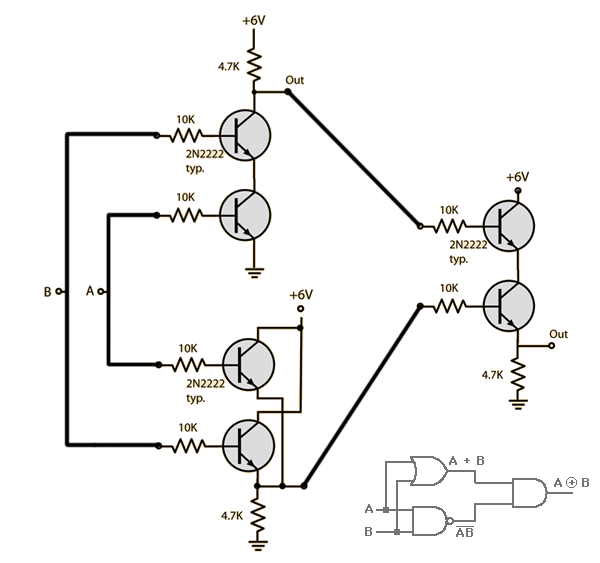
\includegraphics[width=0.25\textwidth,valign=c]{img/exp3/fig1}
			\label{fig:xor_circuit}
		}
		\caption{\textit{XOR gate}}
	\end{figure}
	
	
	\subsection{XNOR gate}
		The 'Exclusive-NOR' gate circuit does the opposite to the EX-OR gate. It will give a low output if either, but not both of its two inputs are high. The symbol is an EX-OR gate with a small circle on the output. The small circle represents inversion.
		\begin{align*}
			Y &= \overline{A \oplus B}
		\end{align*}		
		Ex-NOR gate is created from AND, NOT and OR gates.The output is high only when both the inputs are same.
		\begin{figure}[ht]
			\centering 
			\subfloat[Symbol]
			{
				\begin{circuitikz} \draw
					(0,0) node[xnor port] (myand1) {}
					(myand1.in 1) node[anchor=east] {A}
					(myand1.in 2) node[anchor=east] {B}
					(myand1.out) node[anchor=west] {Y}
					;
				\end{circuitikz}
				\label{fig:xnor_symbol}
			}	
			\hfill
			\subfloat[Truth Table]
			{
				\begin{tabular}{|c|c|c|}
					\hline
					\multicolumn{2}{|c|}{Input} & Output \\
					\hline
					$A$ & $B$ & $Y=\overline{A\oplus B}$ \\
					\hline
					0 & 0 & 1 \\
					\hline
					0 & 1 & 0 \\
					\hline
					1 & 0 & 0 \\
					\hline
					1 & 1 & 1 \\
					\hline
				\end{tabular}
				\label{fig:xnor_table}
			}
			\hfill
			\subfloat[RTL Design]{
				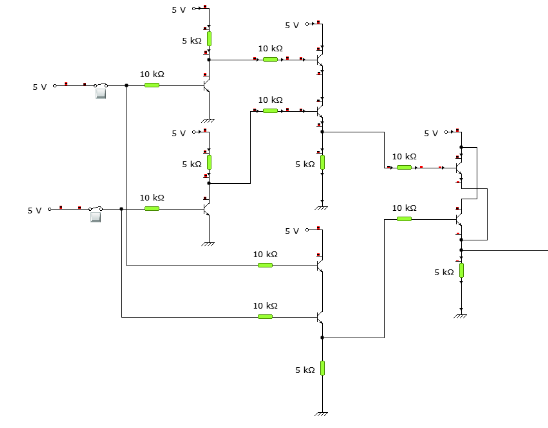
\includegraphics[width=0.25\textwidth,valign=c]{img/exp3/fig2}
				\label{fig:xnor_circuit}
			}
			\caption{\textit{XNOR gate}}
		\end{figure}
		
\section{Procedure}
	\subsection{XOR gate}
		\begin{figure}[ht]
			\centering 
			\subfloat[Simulator 1]{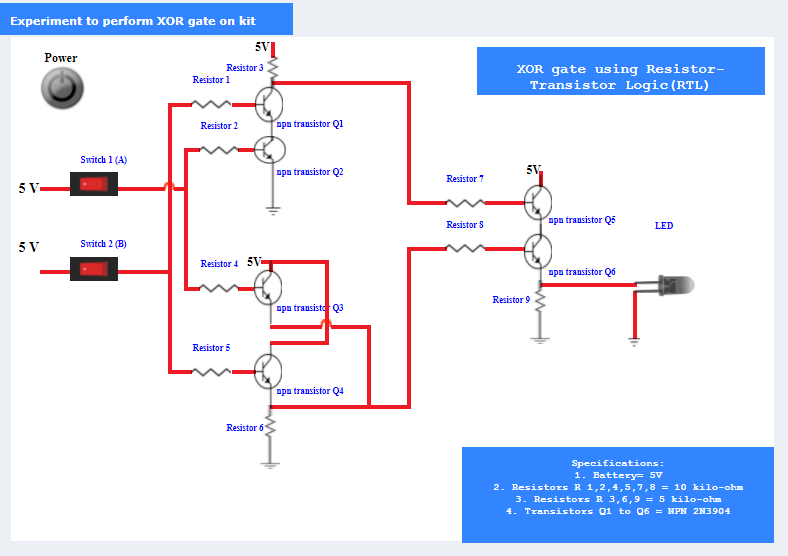
\includegraphics[width=0.45\textwidth,valign=c]{img/exp3/fig3}
				\label{fig:xor_sim:1}}	
			\hfill
			\subfloat[Simulator 2]{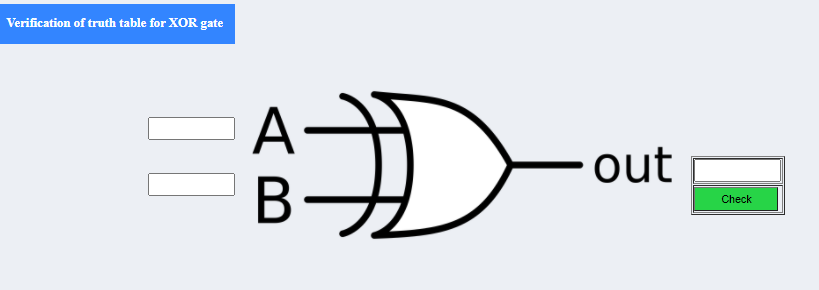
\includegraphics[width=0.4\textwidth,valign=c]{img/exp3/fig4}
				\label{fig:xor_sim:2}}			
			\caption{\textit{Simulator for realizing circuit for XOR gate}}
		\end{figure}
		\subsubsection{Simulator 1}
			\begin{enumerate}
				\tightlist
				\item Connect the supply(+5V) to the circuit.
				\item Press the switches for inputs "A" and "B".			
				\item The bulb glows if one of the switches is ON and one of the switches is OFF else it won't glow.
				\item Repeat step-2 and step-3 for all state of inputs.
			\end{enumerate}
		\subsubsection{Simulator 2}
			\begin{enumerate}
				\tightlist
				\item Enter the Boolean input "A" and "B".
				\item Enter the Boolean output for your corresponding inputs.
				\item Click on "Check" Button to verify your output.			
			\end{enumerate}	

	\subsection{XNOR gate}
		\begin{figure}[ht]
			\centering 
			\subfloat[Simulator 1]{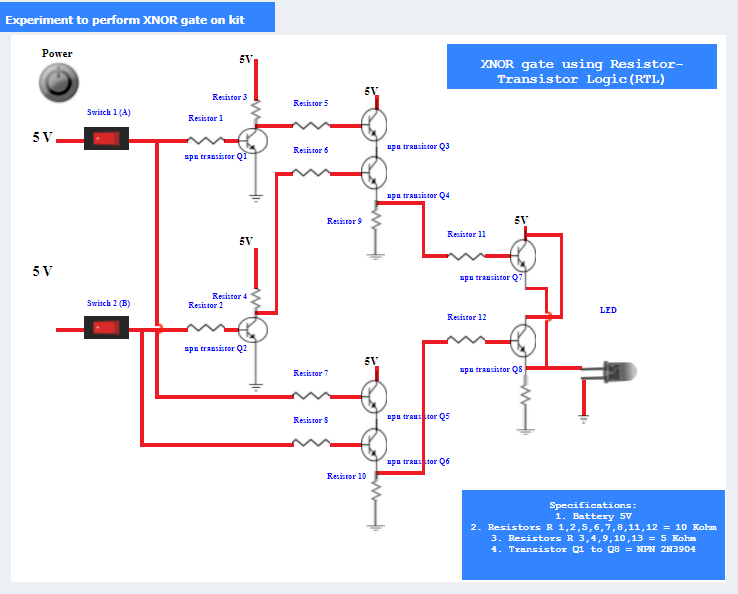
\includegraphics[width=0.45\textwidth,valign=c]{img/exp3/fig5}
				\label{fig:xnor_sim:1}}	
			\hfill
			\subfloat[Simulator 2]{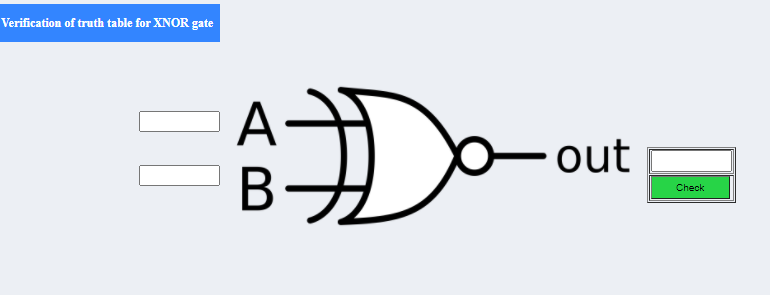
\includegraphics[width=0.4\textwidth,valign=c]{img/exp3/fig6}
				\label{fig:xnor_sim:2}}
			\caption{\textit{Simulator for realizing circuit for XNOR gate}}
		\end{figure}
		\subsubsection{Simulator 1}
			\begin{enumerate}
				\tightlist
				\item Connect the supply(+5V) to the circuit.
				\item Press the switches for inputs "A" and "B".			
				\item The bulb glows if both the switches are ON or if both the switches are OFF else it won't glow.
				\item Repeat step-2 and step-3 for all state of inputs.
			\end{enumerate}
		\subsubsection{Simulator 2}
			\begin{enumerate}
				\tightlist
				\item Enter the Boolean input "A" and "B".
				\item Enter the Boolean output for your corresponding inputs.
				\item Click on "Check" Button to verify your output.			
			\end{enumerate}

\section{Observations}
	\subsection{XOR gate}
			\begin{figure}[ht]
				\centering 
				\subfloat[If the Inputs are alternative, LED is ON]{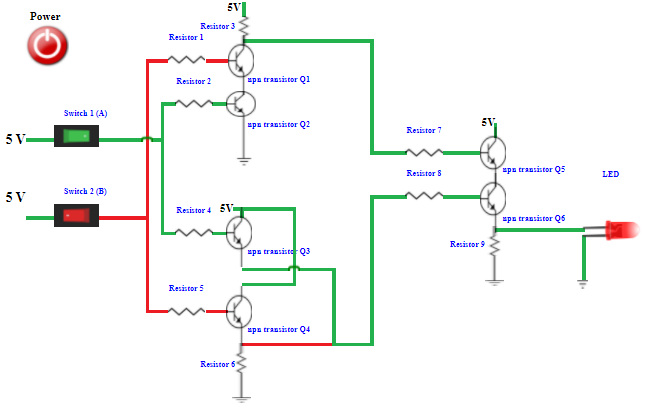
\includegraphics[width=0.45\textwidth,valign=c]{img/exp3/fig7}
					\label{fig:xor_obs:1}}	
				\hfill
				\subfloat[If both Inputs are same, LED is OFF]{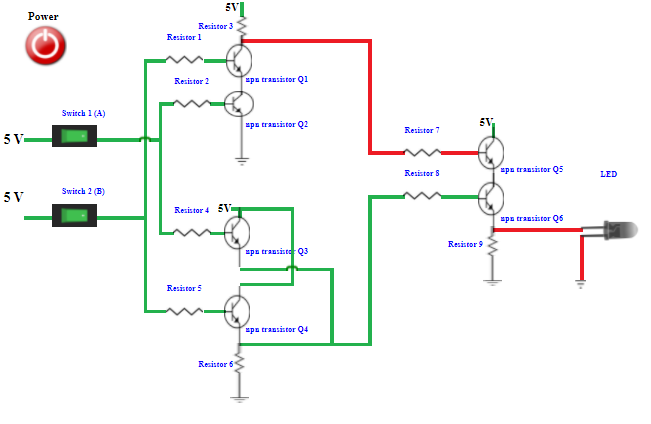
\includegraphics[width=0.45\textwidth,valign=c]{img/exp3/fig8}
					\label{fig:xor_obs:2}}			
				\caption{\textit{Observations for different Input Values}}
			\end{figure}
			\begin{figure}[h]
				\centering
				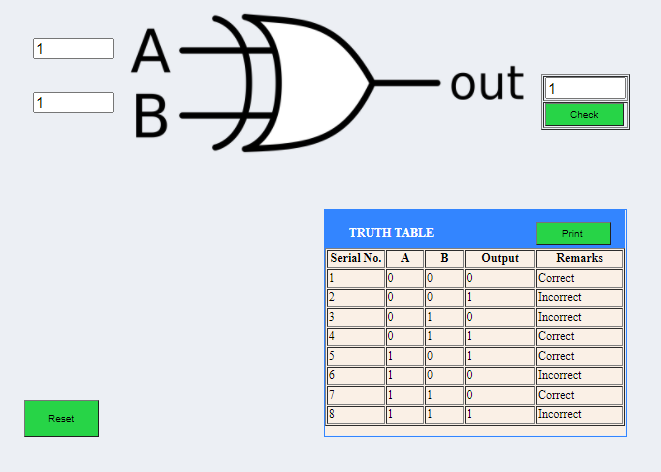
\includegraphics[width=0.85\linewidth]{img/exp3/fig9}
				\caption{\textit{Observations for verification of Truth Table of the XOR gate}}
				\label{fig:xor_obs_2}
			\end{figure}

\pagebreak
	\subsection{XNOR gate}
			\begin{figure}[ht]
				\centering 
				\subfloat[If the Inputs are alternative, LED is OFF]{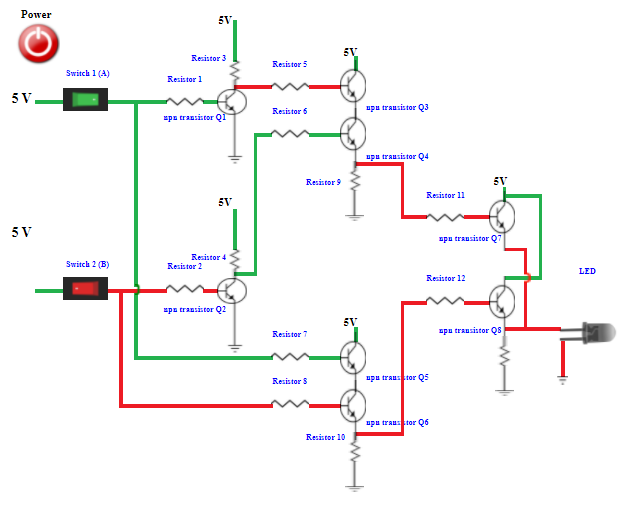
\includegraphics[width=0.45\textwidth,valign=c]{img/exp3/fig10}
					\label{fig:xnor_obs:1}}	
				\hfill
				\subfloat[If both Inputs are same, LED is ON]{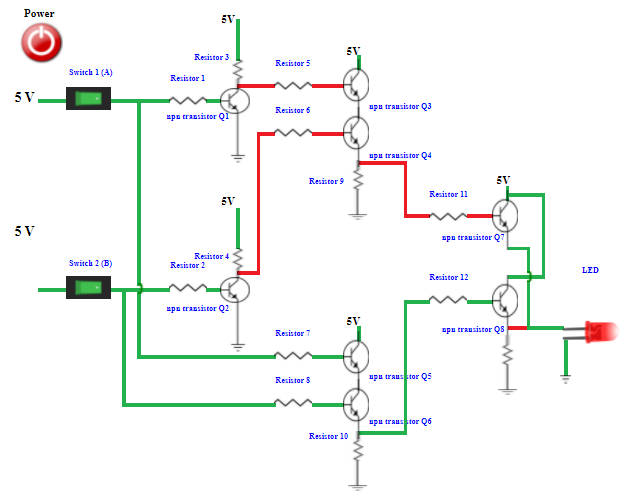
\includegraphics[width=0.45\textwidth,valign=c]{img/exp3/fig11}
					\label{fig:xnor_obs:2}}
				\caption{\textit{Observations for different Input Values}}
			\end{figure}
			\begin{figure}[h]
				\centering
				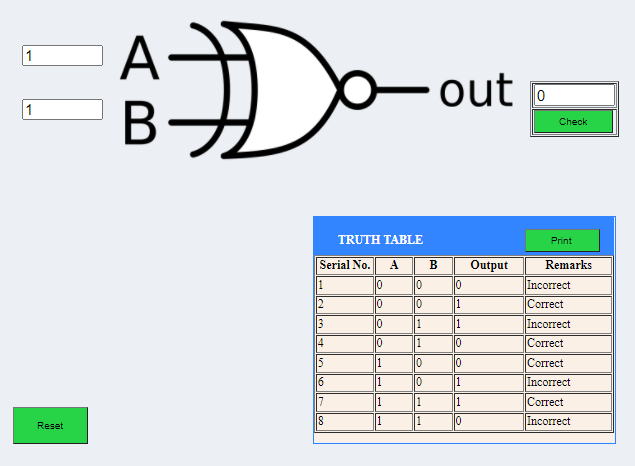
\includegraphics[width=0.85\linewidth]{img/exp3/fig12}
				\caption{\textit{Observations for verification of Truth Table of the XNOR gate}}
				\label{fig:xnor_obs_2}
			\end{figure}
			
\section{Precautions}
	\begin{enumerate}
		\tightlist
		\item Make the connections when power supply is OFF.
		\item Ensure that the connections are tight.
		\item Change the status of inputs only when power supply is OFF.
	\end{enumerate}